\documentclass[12pt, letterpaper]{elsarticle}
\usepackage[utf8]{inputenc}
\usepackage{graphicx}

\title{Neutronics aspects of the FESS-FNSF}
\author[wisc]{Andrew Davis\corref{cor1}}
\ead{andrew.davis@wisc.edu}
\author[wisc]{Moataz Harb}
\ead{moataz.harb@wisc.edu}
\author[wisc]{Laila El-Guebaly}
\ead{elguebaly@wisc.edu}
\author[wisc]{Paul PH Wilson}
\ead{paul.wilson@wisc.edu}
\author[wisc]{Ed Marriott}
\ead{marriott@wisc.edu}
\ead[url]{http://cnerg.wisc.edu}
\cortext[cor1]{Corresponding author}

\address[wisc]{1500 Engineering Drive, Madison, WI 53706}
 
\begin{document}
 
\begin{abstract}
The neutronic aspects of the Fusion Energy System Studies (FESS) Fusion Neutron Sceince 
Facility (FNSF) were studied. Fourteen different sector configurations were investigated to 
determine the impact which each has upon the Tritium Breeding Ratio (TBR) of the whole machine.

\end{abstract}

\begin{titlepage}
\maketitle
\end{titlepage}


\section{Introduction}
The Fusion Energy Systems Studies (FESS) Fusion Neutron Science Facility (FNSF) 
is considered an essential element of the US fusion roadmap that displays a strategic 
pathway from ITER, to US DEMO, and eventually to the first commercial power plant. This paper
describes the stages of nuclear analysis that serve to prove the radiation derived atributes
of the system.

\subsection{Configuration}
The systems studies calculations performed have lead to a radial build which defines the material
basis for these calculations.
\subsection{Full 3D Build}
The radial build calculation defines the major materials and dimensions that produce the 
3D assembley CAD model shown in Figure \ref{fig:cad_fess_fnsf_3d}.
\begin{figure}[ht!]
  \centering
  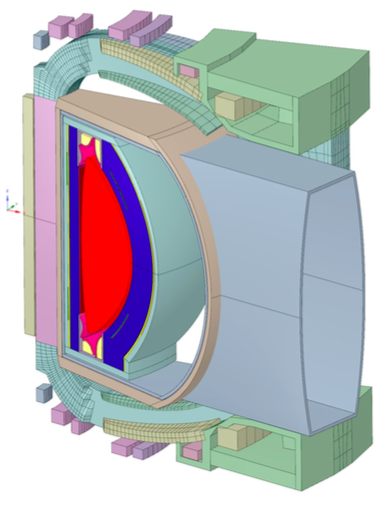
\includegraphics[scale=0.8]{plots/fess_fnsf_3d_cad.png}
  \caption{The full 3D CAD model of a single FESS-FNSF sector}
  \label{fig:cad_fess_fnsf_3d}
\end{figure}
\section{Neutron Source Modelling}
\section{Neutron Wall Load}
\section{TBR Scan}
\section{SDR Calculations}
\subsection{SDR}
\subsection{Decay Heat}
\end{document}